\documentclass[12pt]{article}
\title{ECE 11L Lab Report 1}

\author{Lawrence Liu}
\usepackage{graphicx}
\usepackage{amsmath}
\usepackage{subcaption}
\usepackage{array}

\begin{document}
\begin{titlepage}
   \begin{center}
       \vspace*{1cm}

       \textbf{EE 11L: Circuits Laboratory I}

       \vspace{2cm}

       \textbf{Experiment \#3}\\
       \textbf{Experiment 3: Transient Response of the 1st-Order
Circuits}

            
       \vspace{4cm}
     
            
       Name: Lawrence Liu\\
		UID: 405749034\\
		Due Date: Nov. 11, 2100
            
   \end{center}
\end{titlepage}
\section*{Objectives}
To understand and investigate the natural and step response of first order capacitive and inductive circuits. To design a first-order circuit with certain characteristics. To analyze initial conditions within a circuit containing inductors and capacitors 
\section*{Theory}
\textbf{Capacitors}
The i-v relation of a capacitor is
$$i=C\frac{dv}{dt}$$
The voltage across a capacitor cannot change unless infinite current is applied
\\
\textbf{RC Circuits}
when a capacitor and a resistor is connected in series with a voltage source $V$ we have the following equation for the voltage $v_C$ across the capacitor
$$v_C+RC\frac{dv_C}{dt}=V$$
Therefore the response to a step voltages source $V(t)=Vu(t)$ is
$$v_C(t)=V(1-e^{\frac{-t}{RC}})$$
and the time constant is $\tau=RC$ 
\\
\textbf{Inductors} The i-v relation of a capacitor is 
$$V=L\frac{di}{dt}$$
The current across a inductor cannot change unless infinite voltage is applied. 
\\\\
\textbf{RL circuits} 
when a capacitor and a resistor is connected in series with a voltage source $V$ we have the following equation for the voltage $v_l$ across the capacitor
$$v_l+\frac{L}{R}\frac{dv_l}{dt}=V$$
Therefore, the response to a step voltage source $V(t)=Vu(t)$ is
$$v_C(t)=V(1-e^{-\frac{R}{L}t})$$
\pagebreak
\section*{Lab 1: Experiment Setup}
\begin{figure}[h]
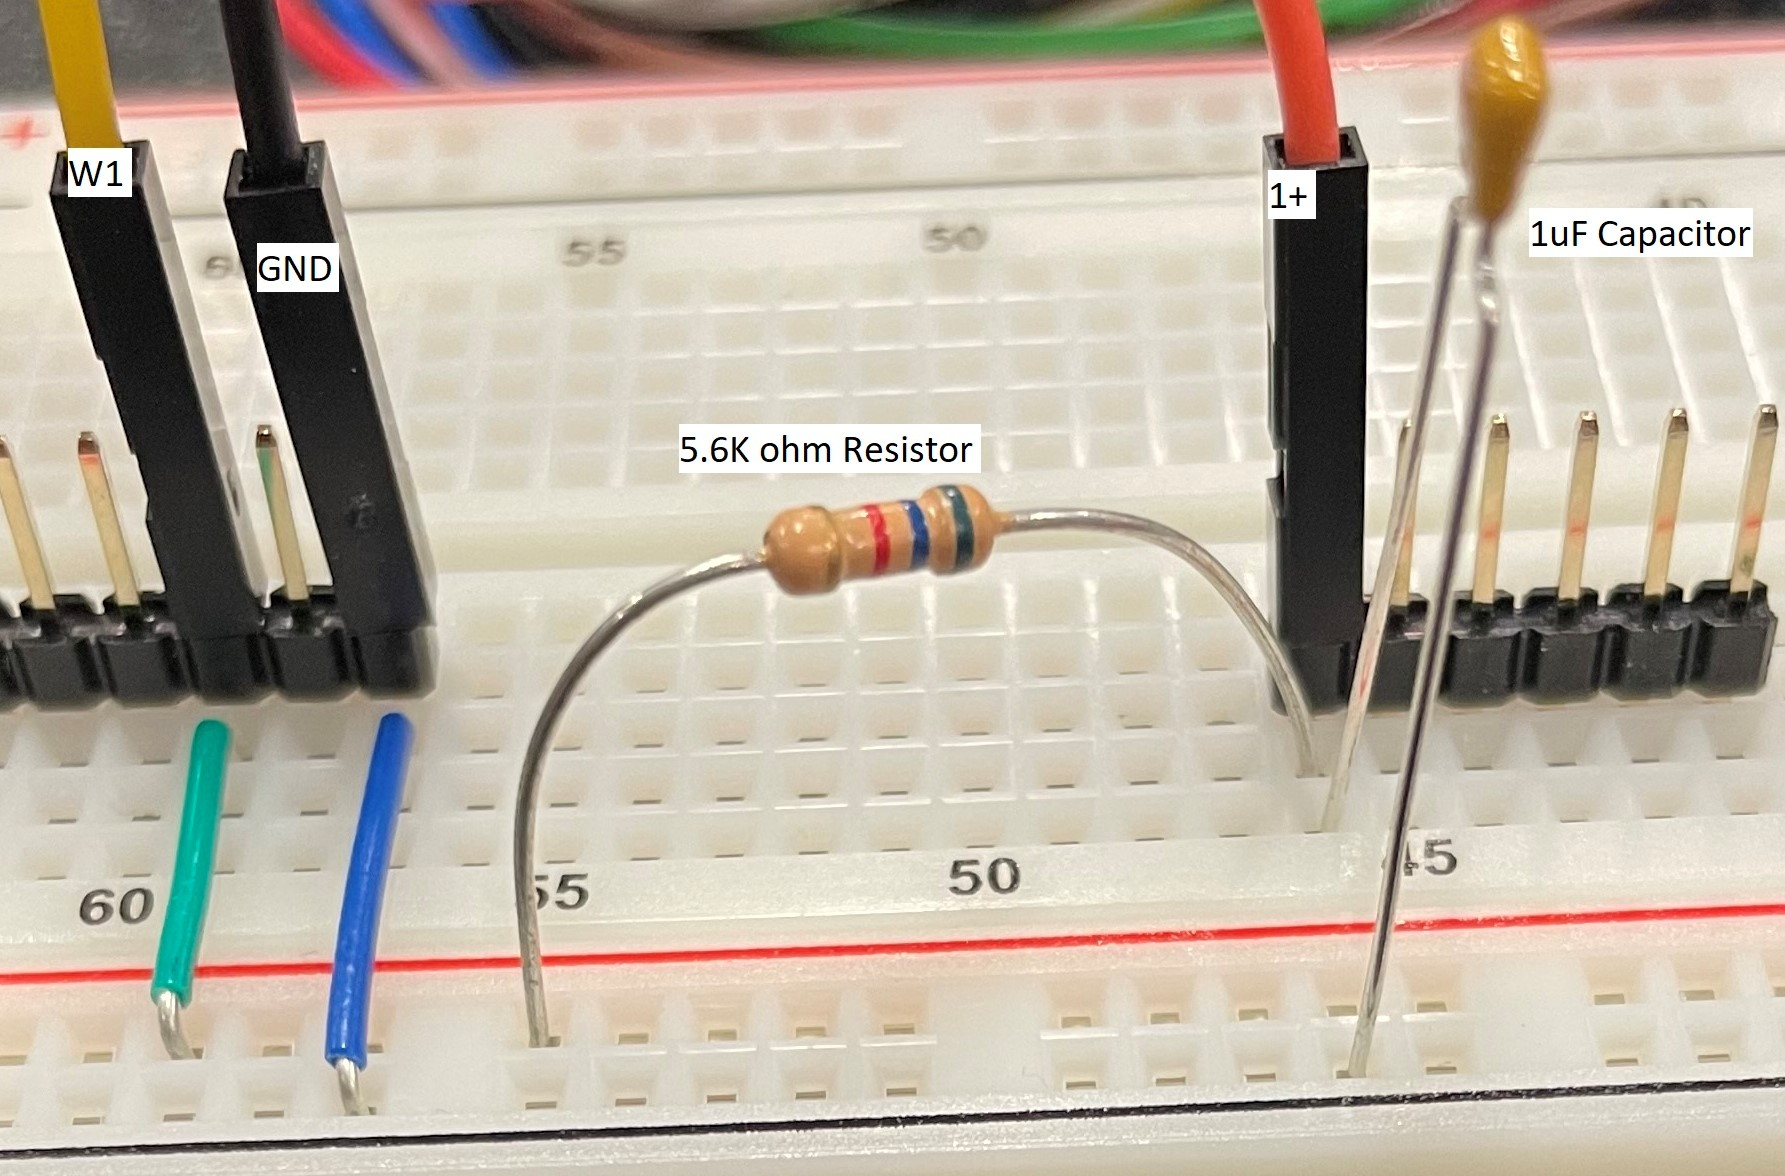
\includegraphics[width=8cm]{Lab1}
\centering
\caption{Lab 1 Setup}
\end{figure}
\section*{Lab 1: Measurement}
The measured time constant is $531.56\mu s$
\begin{figure}[h]
\includegraphics[width=10cm]{Problem 1 Fig}
\centering
\caption{Measurements from the oscilloscope for Lab 1, C1:VC the voltage response of the capacitor}
\end{figure}
\section*{Lab 1: Discussion}

The experimental time constant is $531.56\mu s$ and the theoretical time constant is $560\mu s$. The difference between these two values is $8.35\%$
\\\\
Since the resistor is in parallel with the capacitor, the resistor's voltage response is $V_r=V(t)-V_c(t)$ where $V_r$ is the voltage across the capacitor and $V_c(t)$ is the voltage across the capacitor. Therefore, as the capacitors voltage increases, the resistor's voltage decreases, and vice versa. 
\\\\

Increasing the sampling rate increases the resolution of the signal. This
allows for a more accurate reading for the time constant.
\\\\
When you increase the frequency of the input, the signal begins to be unable to reach the theoretical steady state voltage.

\pagebreak
\section*{Lab 2: Experiment Setup}
\begin{figure}[h]
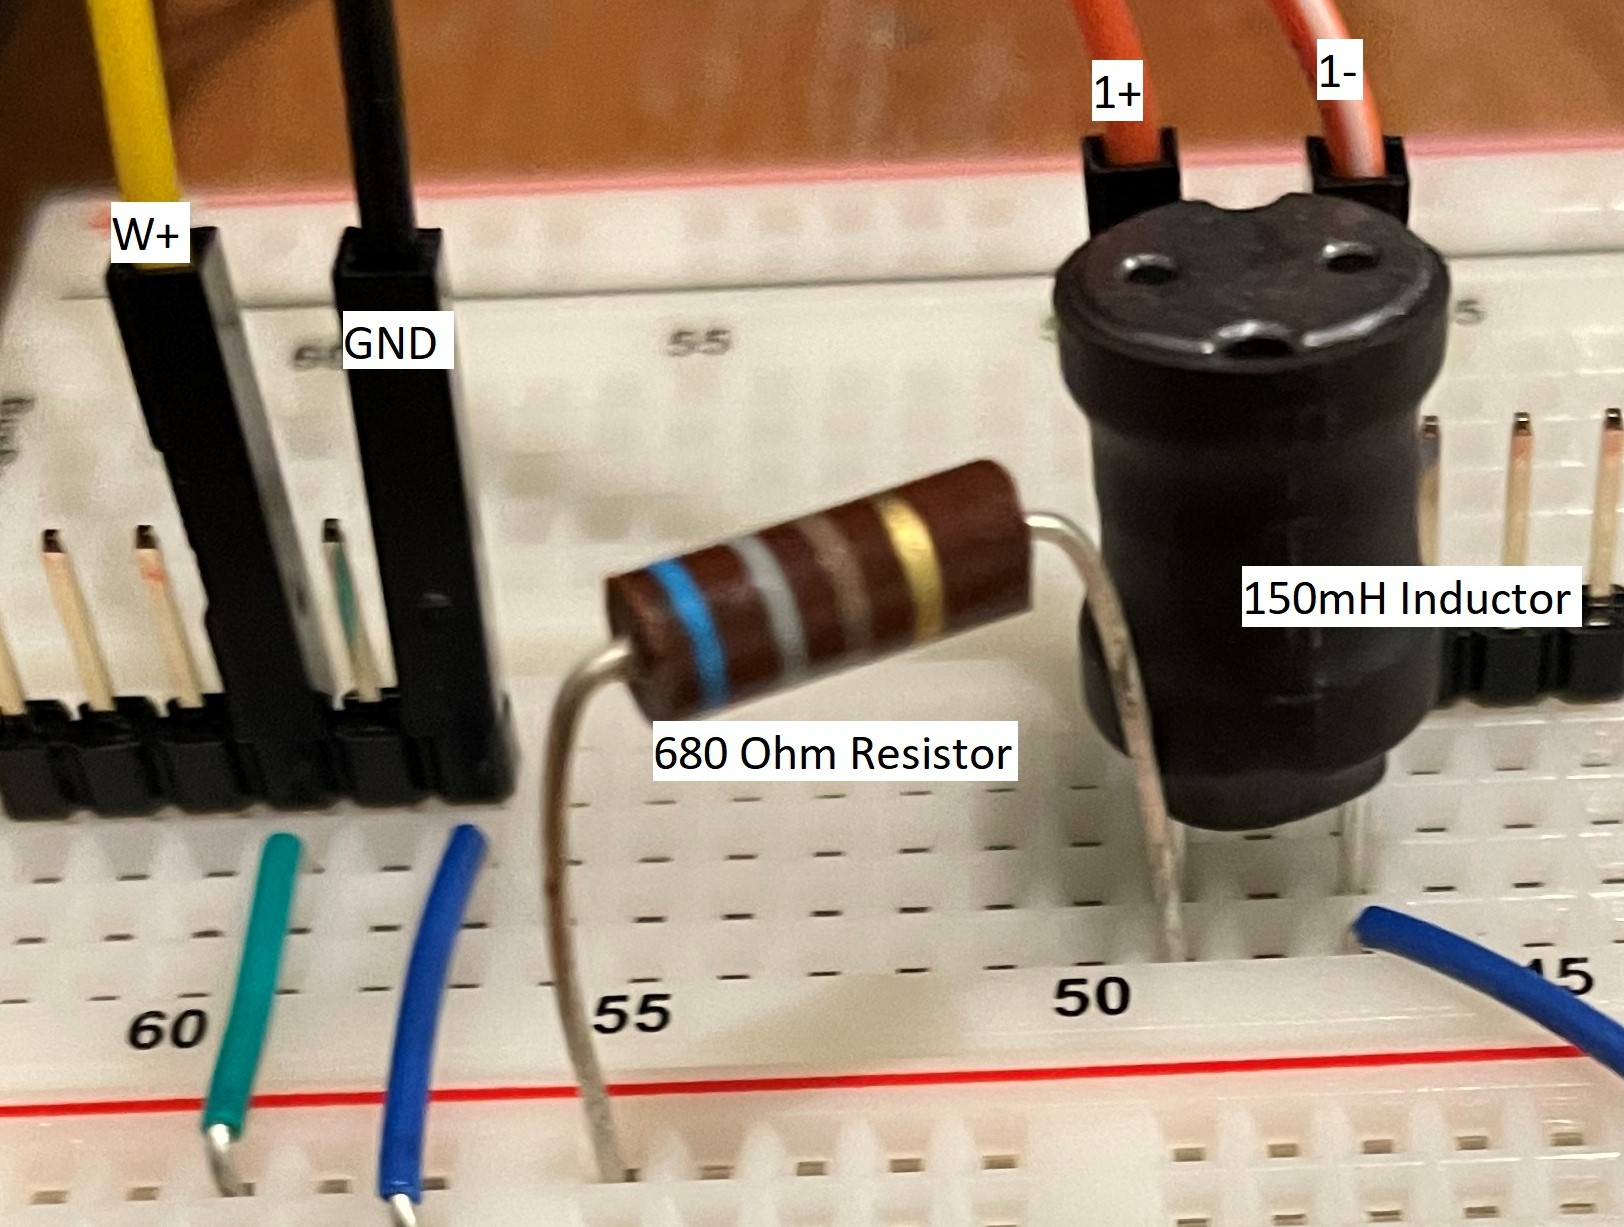
\includegraphics[width=8cm]{Lab2}
\centering
\caption{Lab 2 Setup}
\end{figure}
\section*{Lab 2: Measurement}
The measured time constant is $178.784\mu s$
\begin{figure}[h]
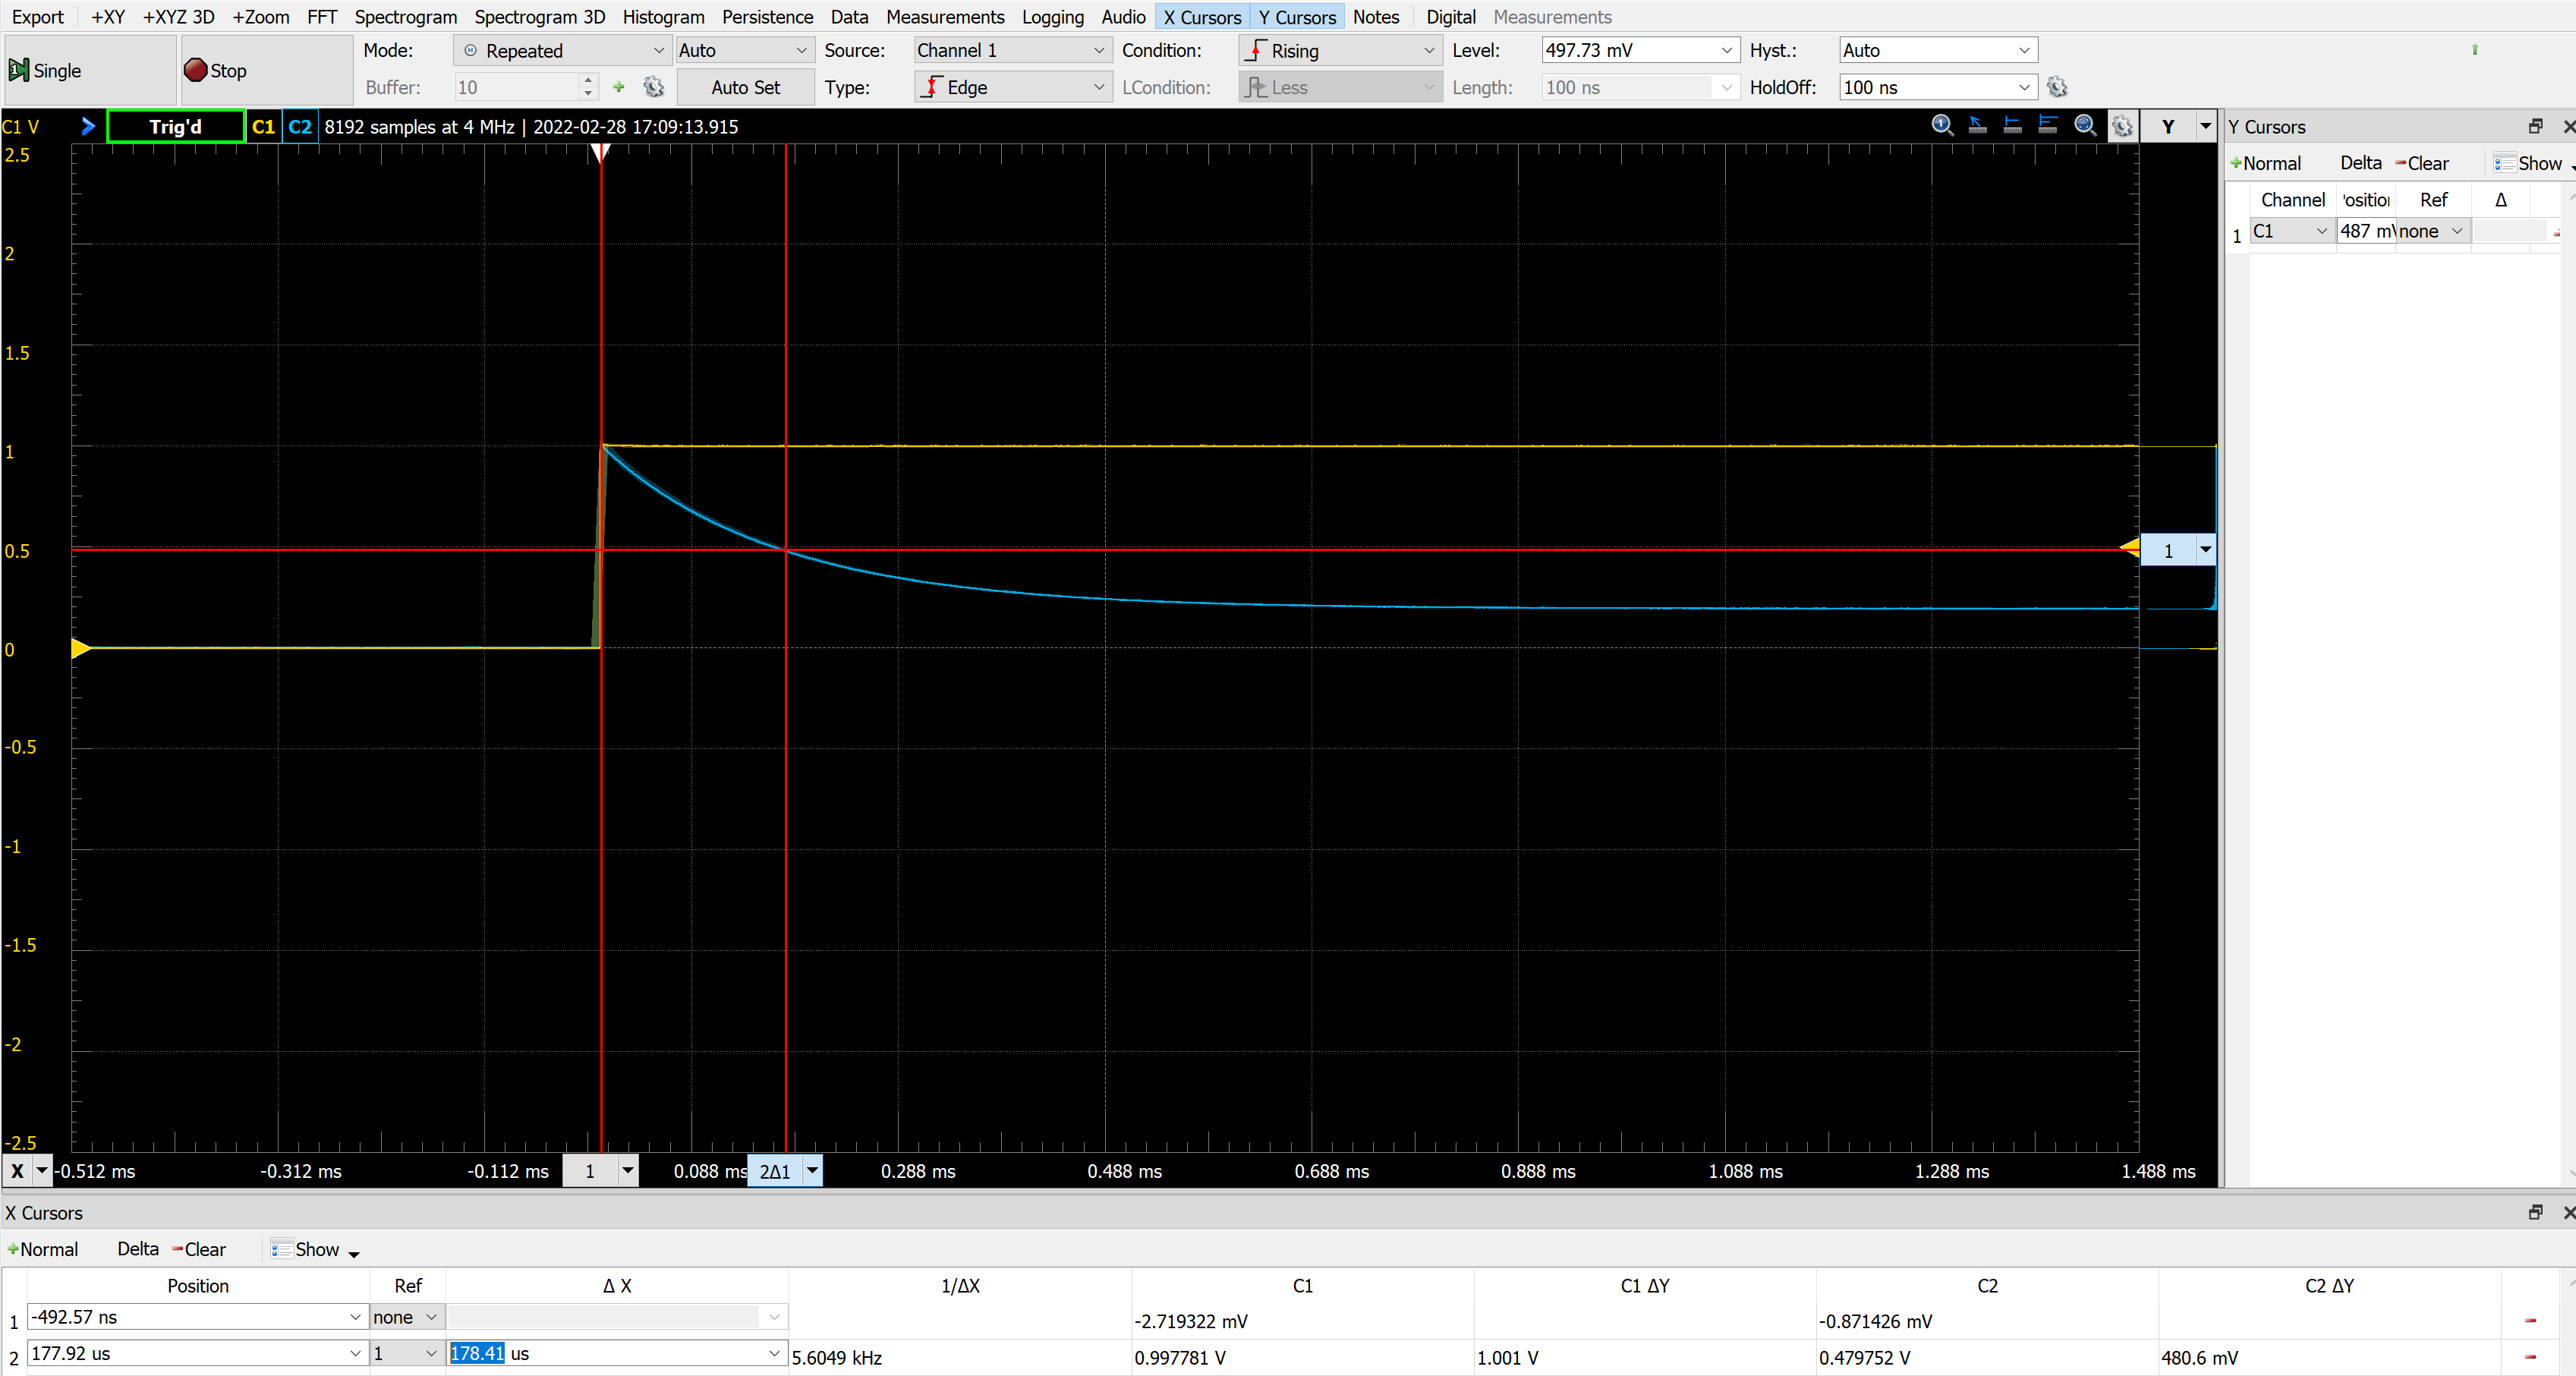
\includegraphics[width=10cm]{Problem 2fig}
\centering
\caption{Measurements from the oscilloscope for Lab 1, C1:VL the voltage response of the inductor}
\end{figure}
\section*{Lab 2: Discussion}

The measured internal resistance of the inductor is $159.5\Omega$, therefore the theoretical $178.784\mu s$. and the measured time constant is $178.41\mu s$ The difference between these two values is $0.2\%$
\\\\
Yes the internal resistance must be considered, since the steady state voltage is 0.19V not 0 volts as it should be theoretically.
\\\\
In the RL circuit the voltage jumps and slowly falls back down when presented with a unit step input. In a RC circuit, the current slowly increases when presented with a unit step input
\pagebreak
\section*{Lab 3: Experiment Setup}
\begin{figure}[h]
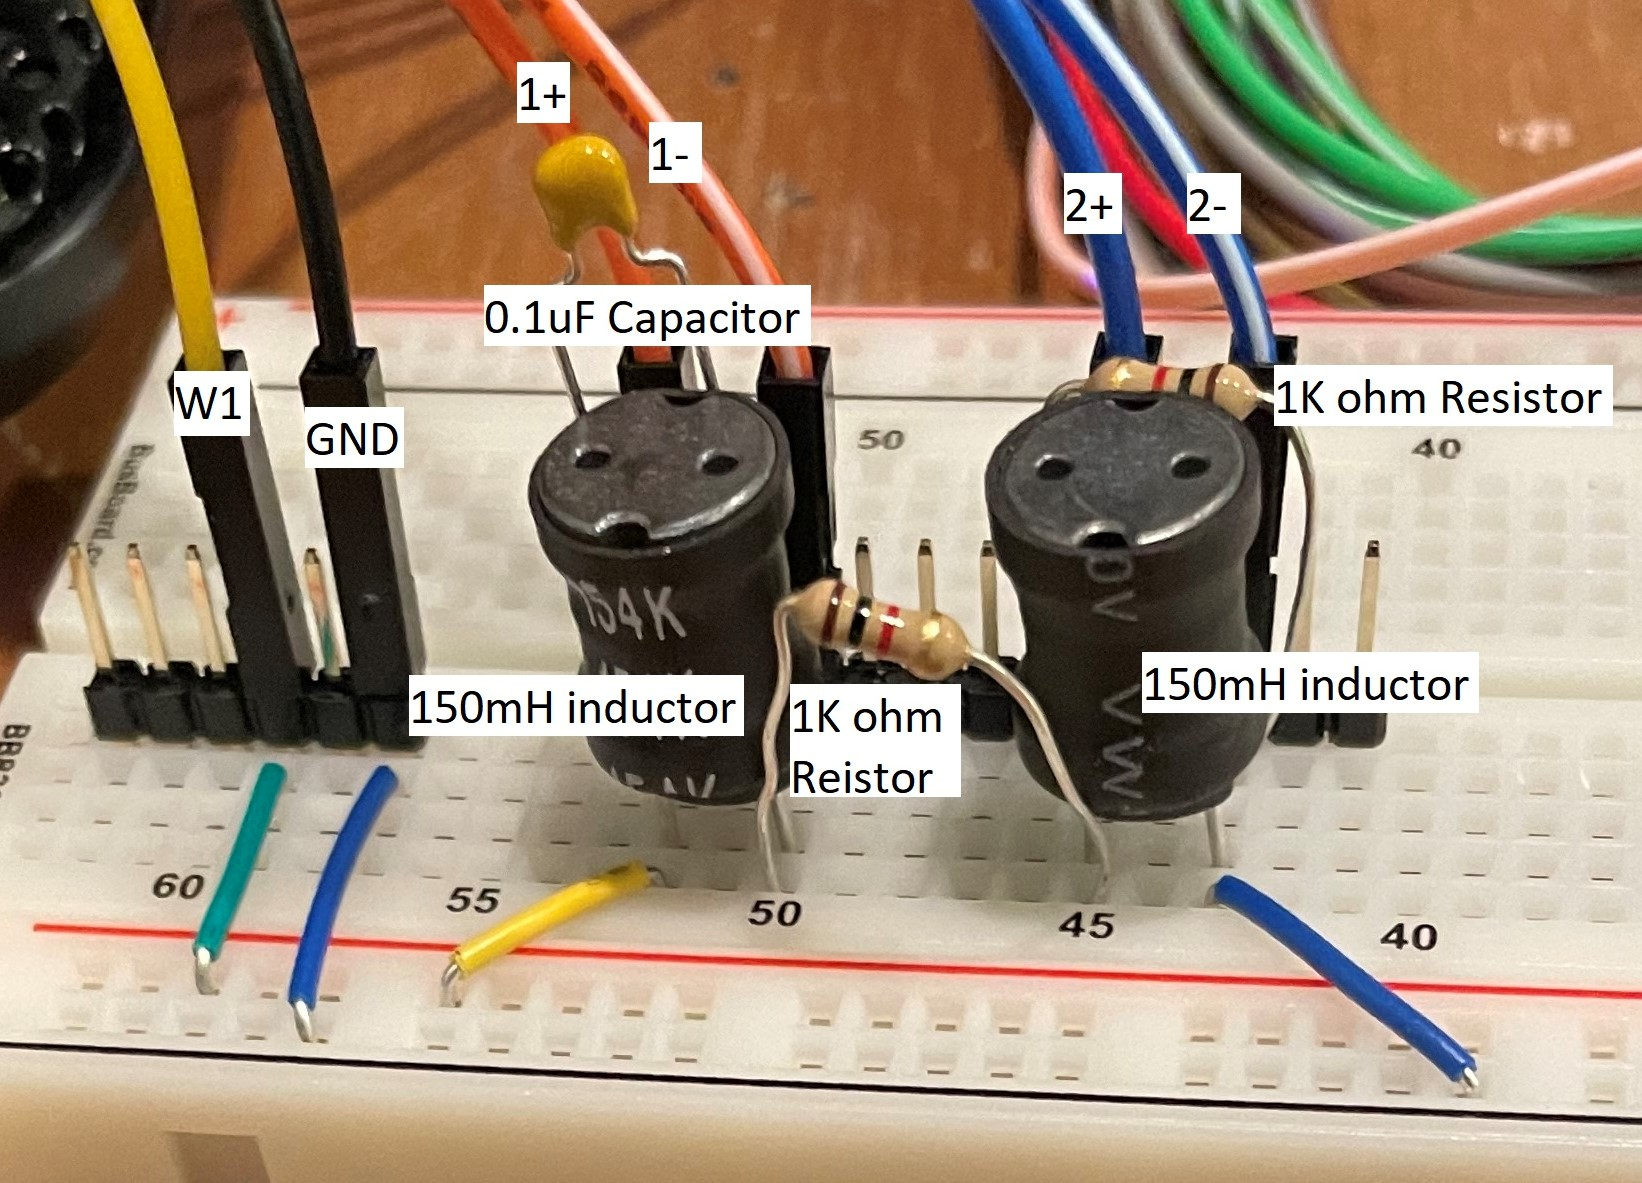
\includegraphics[width=8cm]{Lab3}
\centering
\caption{Lab 3 Setup}
\end{figure}
\section*{Lab 3: Measurement}
\begin{center}
$$V_{c1}(t)$$
\begin{tabular}{|c|c|c|c|}
\hline
& $t=0^-$ & $t=0^+$ & $t=\infty$\\
\hline
Theoretical & 0V& 0V& 0V\\
\hline
Measured & 0.3687V & 0.3682V & 0.2583V\\
\hline
\end{tabular}

$$V_{R1}(t)$$
\begin{tabular}{|c|c|c|c|}
\hline
& $t=0^-$ & $t=0^+$ & $t=\infty$\\
\hline
Theoretical & 3V& 2.5V & 2V\\
\hline
Measured &2.274V  &1.769V  & 1.5138V  \\
\hline
\end{tabular}

$$V_{R2}(t)$$
\begin{tabular}{|c|c|c|c|}
\hline
& $t=0^-$ & $t=0^+$ & $t=\infty$\\
\hline
Theoretical & 0V& -0.5V & 0V\\
\hline
Measured &0.325V  &-0.201V  & 0.215V  \\
\hline
\end{tabular}
\end{center}
\section*{Lab 3: Discussion}
The measured voltages varied significantly from the predicted voltage because of the internal resistance in the inductor and capacitor.
\pagebreak
\section*{Lab 4: Experiment Setup}
\begin{figure}[h]
\includegraphics[width=8cm]{Lab4}
\centering
\caption{Lab 4 Setup}
\end{figure}
\section*{Lab 4: Measurement}
The measured time constant is $159\mu s$
\begin{figure}[h]
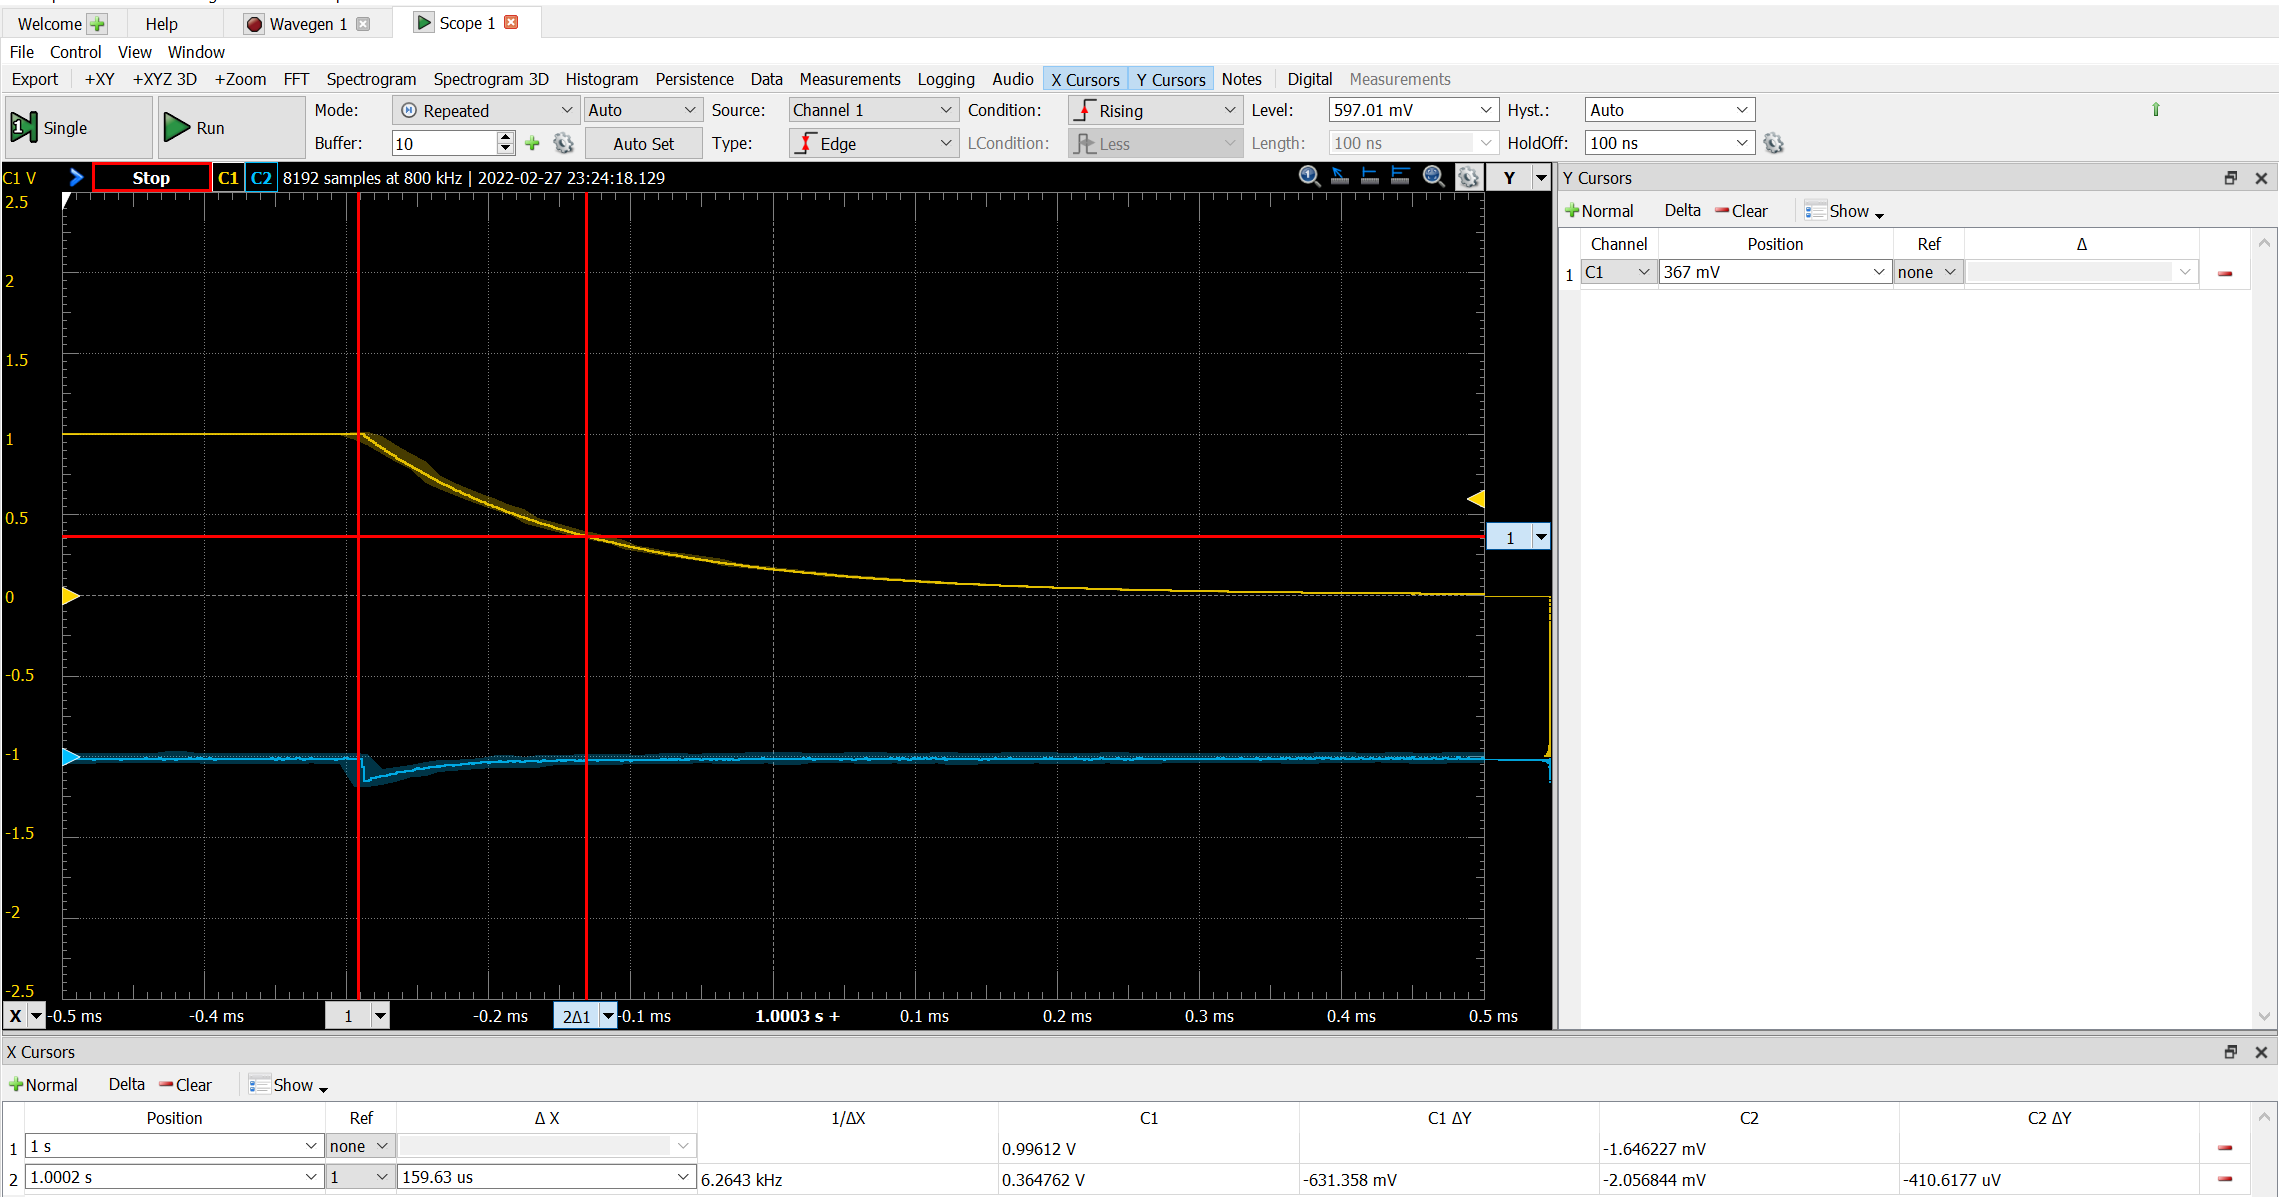
\includegraphics[width=10cm]{Problem 4}
\centering
\caption{Measurements from the oscilloscope for Lab 4, C1:VC the voltage response of the capacitor}
\end{figure}
\pagebreak
\section*{Lab 4: Discussion}
the expected voltage response to start at 1V and then fall to 0 and the theoretical time constant is $165\mu s$. The difference between the measured and expected time constant is $3.6\%$.
\pagebreak
\section*{Lab 5: Setup}
\begin{figure}[h]
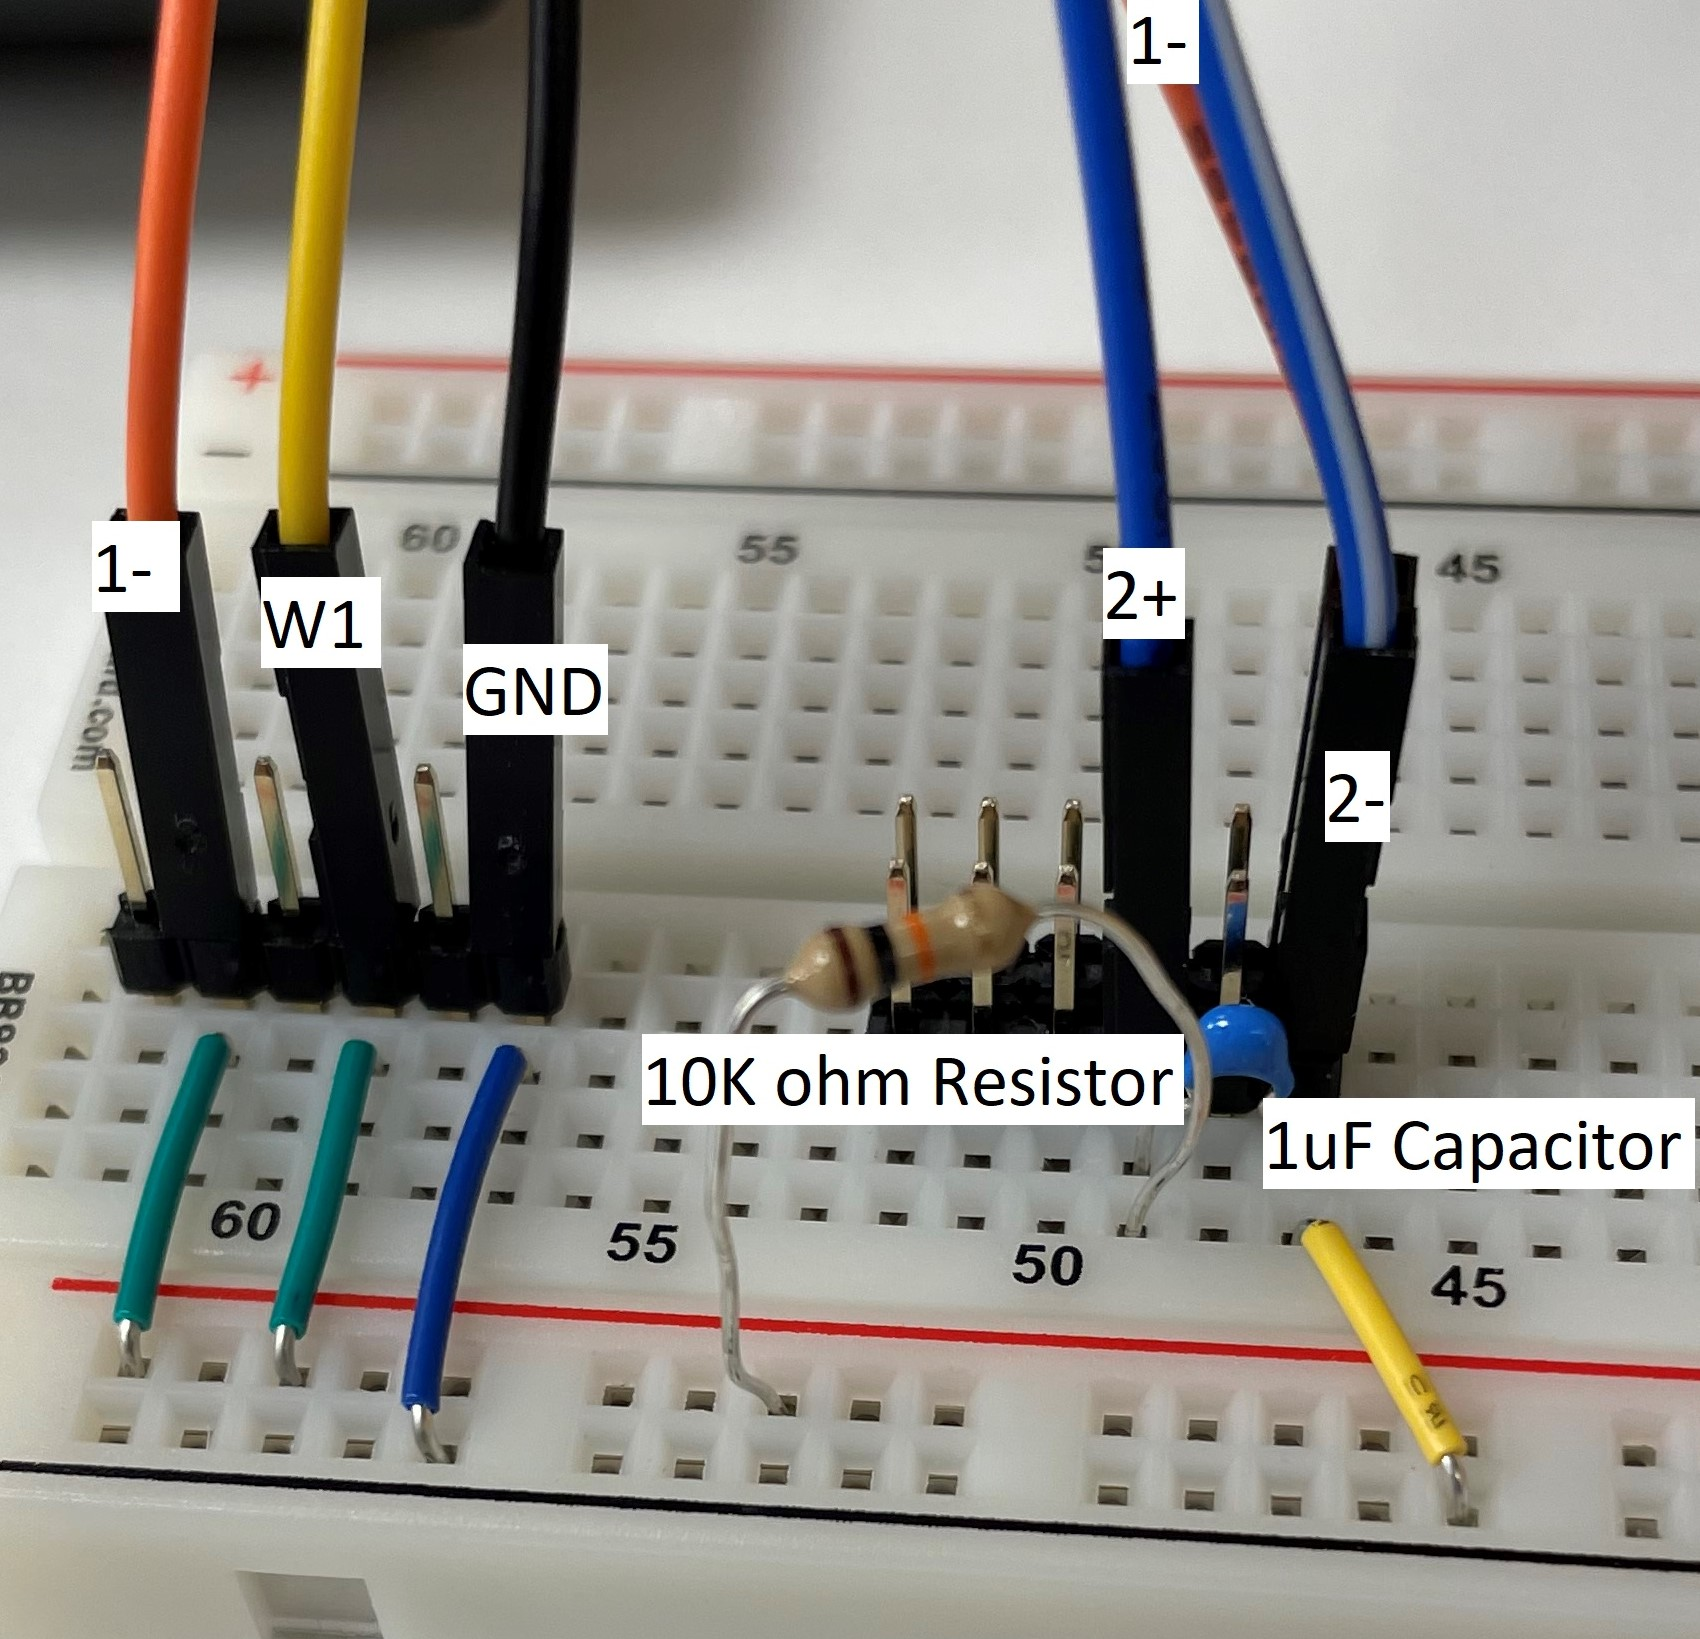
\includegraphics[width=8cm]{Lab 5}
\centering
\caption{Lab 5 Setup}
\end{figure}
\section*{Lab 5: Measurements}
\begin{figure}[h]
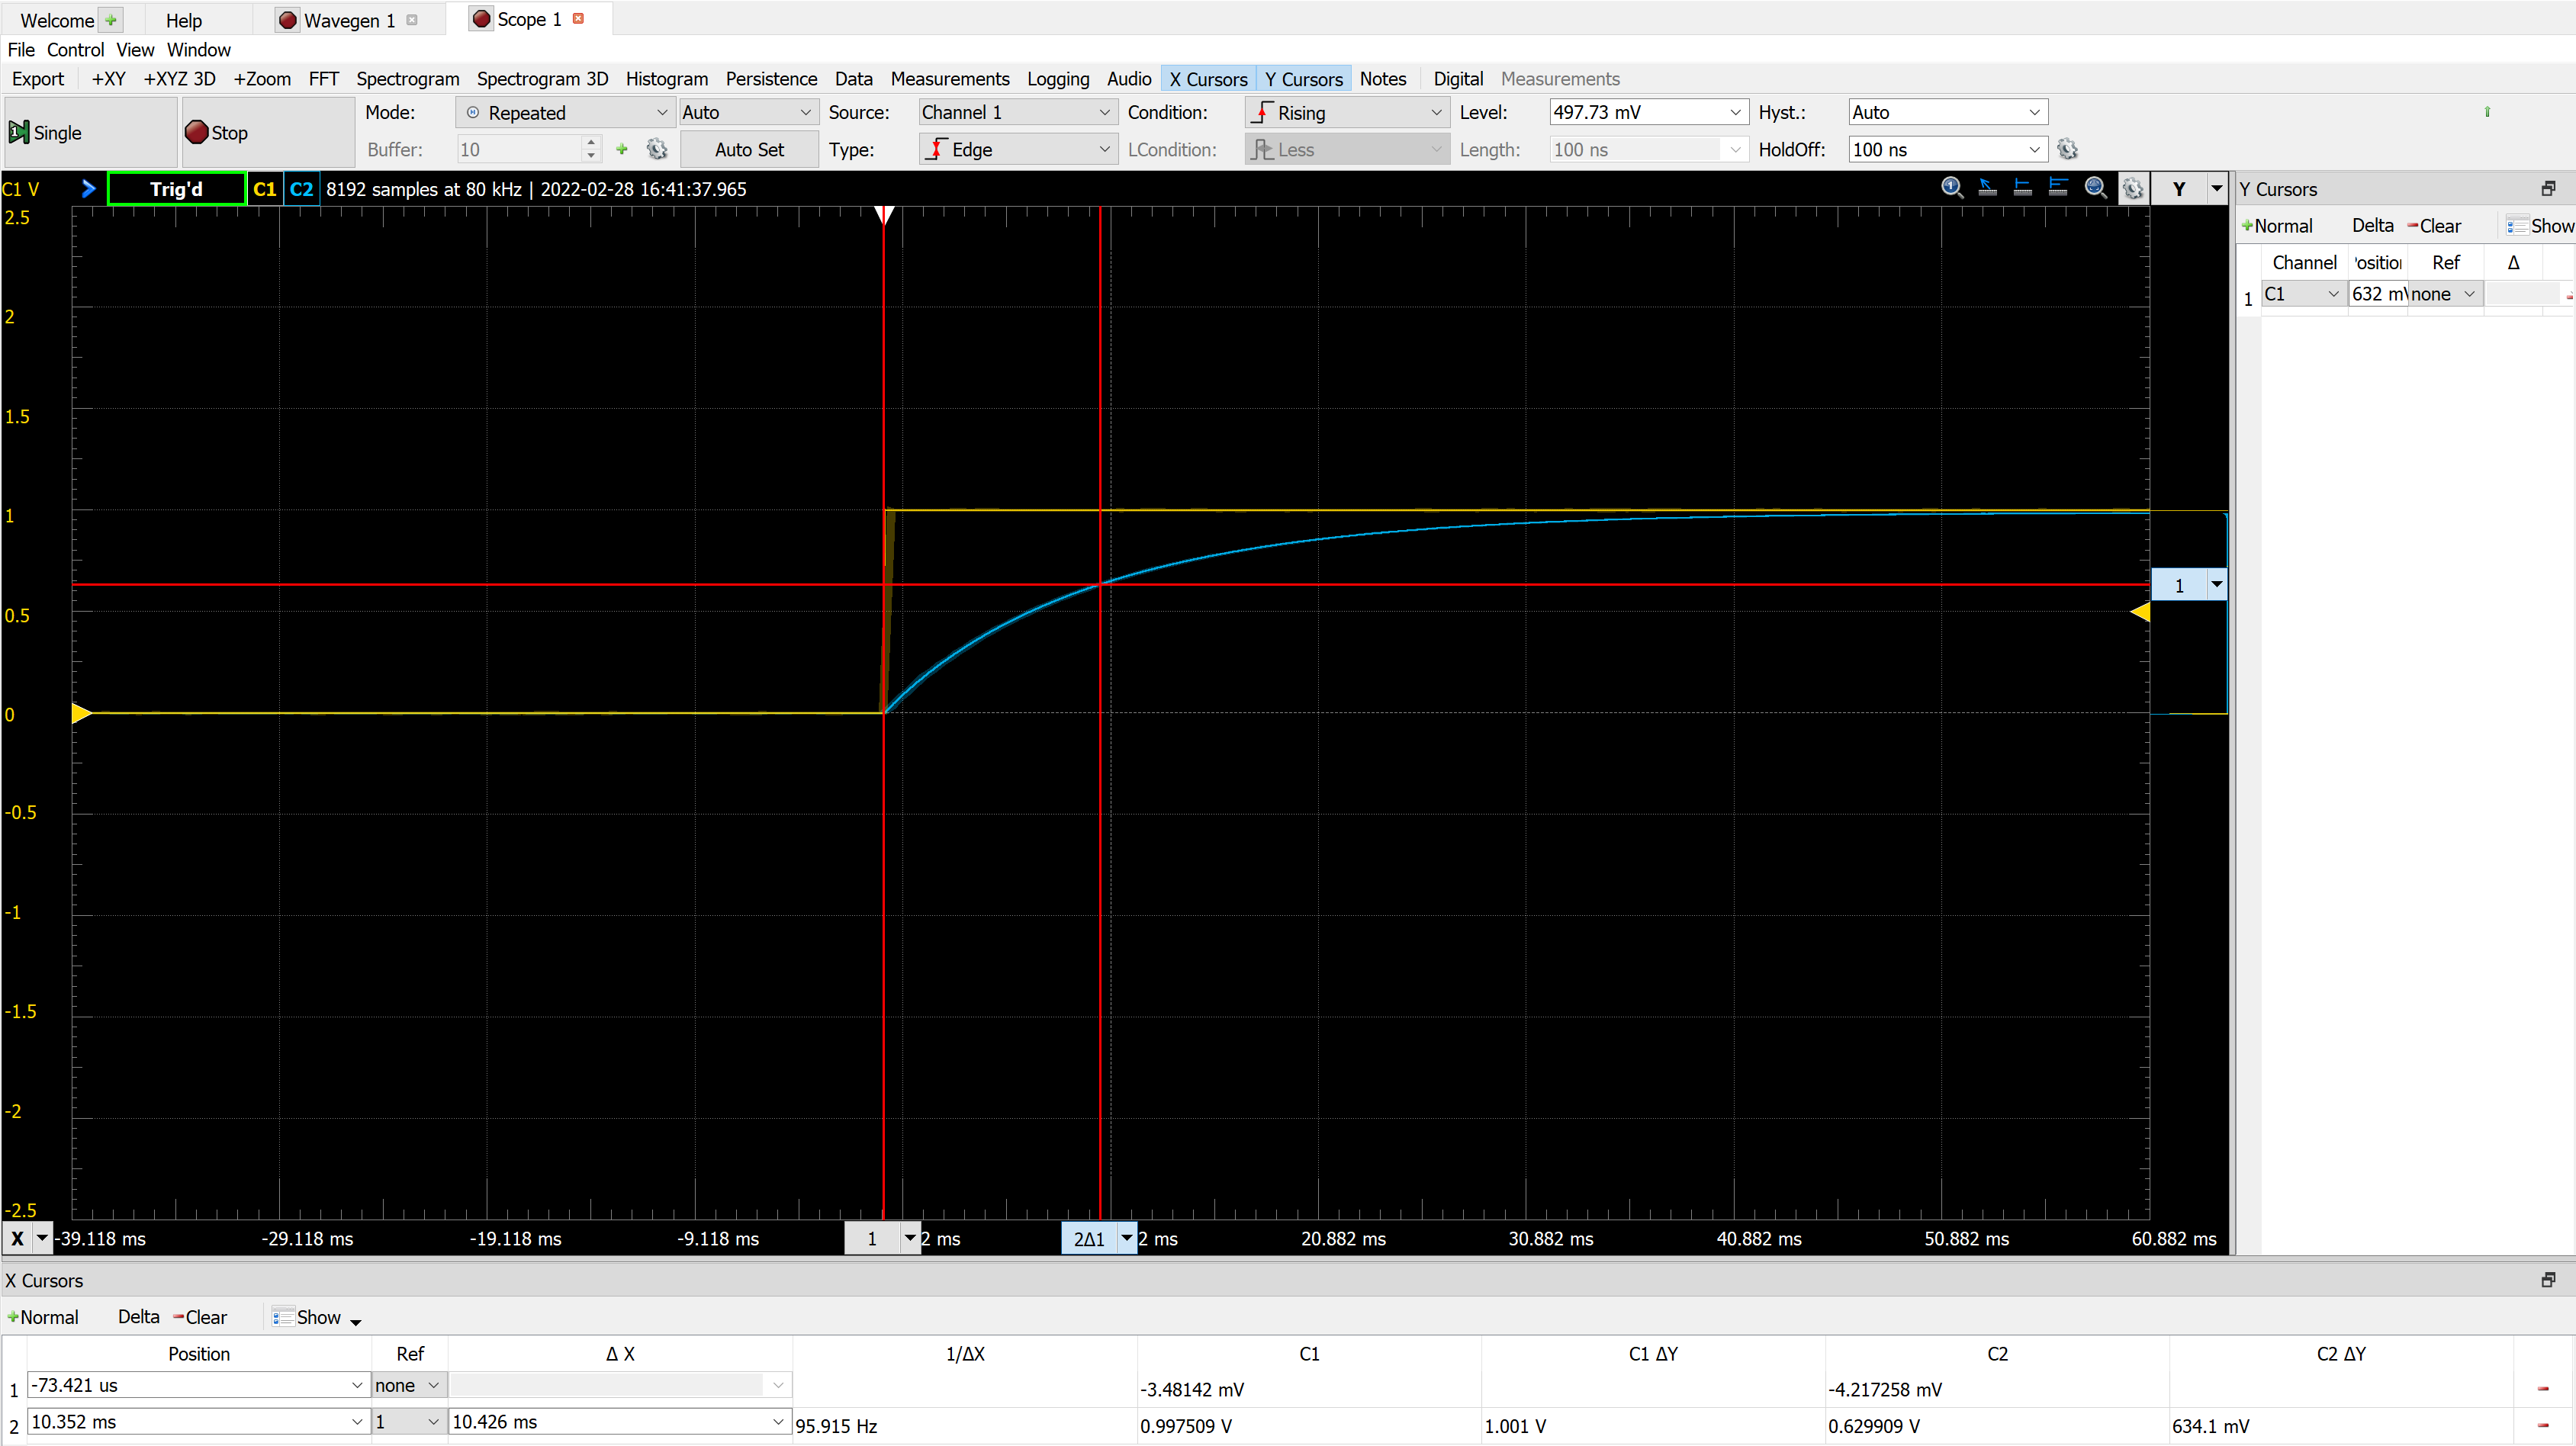
\includegraphics[width=12cm]{Problem 5}
\centering
\caption{Measurements from the oscilloscope for Lab 4, C1:VC the voltage response of the capacitor}
\end{figure}
\pagebreak
\section*{Lab 5: Discussion}
I was able to replicate the given voltage response with a $10K\Omega$ resistor and a $1\mu F$ Capacitor. The time constant of the given voltage response was $9.3274mS$, the voltage response of the circuit I constructed was  $10.426mS$.
\pagebreak
\section*{Conclusion}

We understood and investigated the natural and step response of first order capacitive and inductive circuits. We designed a first-order circuit with certain characteristics. We analyzed initial conditions within a circuit containing inductors and capacitors. 

\end{document}